\documentclass[addpoints]{exam}

% Header and footer.
\pagestyle{headandfoot}
\runningheadrule
\runningfootrule
\runningheader{CS 113 Discrete Mathematics}{HW I: Sets}{Spring 2020}
\runningfooter{}{Page \thepage\ of \numpages}{}
\firstpageheader{}{}{}

% \qformat{{\large\bf \thequestion. \thequestiontitle}\hfill[\totalpoints\ points]}
\boxedpoints
\printanswers

\title{Homework I: Sets\\ CS 113 Discrete Mathematics\\ Habib University -- Spring 2020}
\author{sf06199}  % replace with your ID, e.g. oy02945
\date{29-01-20}
\usepackage{graphicx}

\begin{document}
\maketitle

\begin{questions}


  \question[5]
  Write down $\mathcal{P}(X)$ if 
  $ X = \{ \emptyset, \{\alpha, \beta, \gamma \}, \gamma, \{\{ \alpha, \beta \} \} \}$.
  \begin{solution}
    $\mathcal{P}(X)$ = $\{\emptyset, \{\emptyset\},\{\{\alpha, \beta, \gamma \}\}, \{\gamma\}, \{\{\{ \alpha, \beta \} \}\},\{\emptyset,\{\alpha, \beta, \gamma \}\},\{\emptyset,\gamma\},\{\emptyset,\{\{\alpha, \beta \}\}\},\\ \{ \{\alpha, \beta, \gamma \},\gamma \}, \{ \{\alpha, \beta, \gamma \},\{\{ \alpha, \beta \} \}\}, \{\gamma,\{\{ \alpha, \beta \} \} \},\{\emptyset,\{\alpha, \beta, \gamma \}, \gamma\},\{\emptyset, \gamma, \{\{ \alpha, \beta \} \}\},\\ \{\ \emptyset, \{\alpha, \beta, \gamma \}, \{\{ \alpha, \beta \} \}\} \{\ \{\alpha, \beta, \gamma \}, \gamma, \{\{ \alpha, \beta \} \} \}\},\{ \emptyset, \{\alpha, \beta, \gamma \}, \gamma, \{\{ \alpha, \beta \} \} \} \}$
  \end{solution}

  \question
  \begin{parts}
    \part[5] 
    Assume that RO has asked for your help to generate a set that contains all the possible pairs of DSSE faculty and DSSE courses at Habib University. Describe the sets and set operations that you can use to provide RO the desired set.
    \begin{solution}
      $ C = \{(x,y)\mid x \in DSSE \ faculty \land y \in DSSE \ courses\}$ \\ Where C is the cartesian product of DSSE Faculty and the courses that are offered. \\ Following is the set builder notation form of the two sets x and y, where x belongs to set that contains the DSSE faculty members as its elements whereas y belongs to the set that contains the courses. When we take the Cartesian product of these two, it gives us the possible number of pairs of the faculty and the courses of DSSE. 
    \end{solution}

    \part[5] Imagine that the the operation above is extended to include an additional set that contains all the time slots when a course can be scheduled. Explain the outcome of the obtained set.
    \begin{solution}
     Here, we will find the Cartesian product of C (cartesian product of DSSE Faculty and the courses) and the time slots (D) . \\ 
    $ C \times D = \{(x,y,z) \mid x \in  DSSE Faculty \land y \in DSSE course \land z \in time slots \} $ \\ 
    The final outcome would be the ordered pairs of (x,y,z) where x indicates DSSE  Faculty , y indicates DSSE  courses and z indicates time slots. 
      
    \end{solution}
  \end{parts}
  
  \question
  The \textit{symmetric difference} of two sets $A$ and $B$ is defined as $A\oplus B = (A-B) \cup (B-A)$. It is also known as the \textit{disjunctive union} as it contains all those elements which are in either of those sets, but not in their intersection. 
  \begin{parts}
    \part[5] Prove that $A\oplus B = (A \cup B)-(A \cap B).$
    \begin{solution}
      By definition we know,  $A\oplus B = (A-B) \cup (B-A)$ \\
      So taking left hand side as $(A-B) \cup (B-A)$ and right hand side as $(A \cup B)-(A \cap B)$ \\ 
      Figure \ref{fig:Venn Diagram} proves that $A\oplus B = (A-B) \cup (B-A) =  (A \cup B)-(A \cap B) $
      
    \end{solution}
        \begin{figure}[h!]
          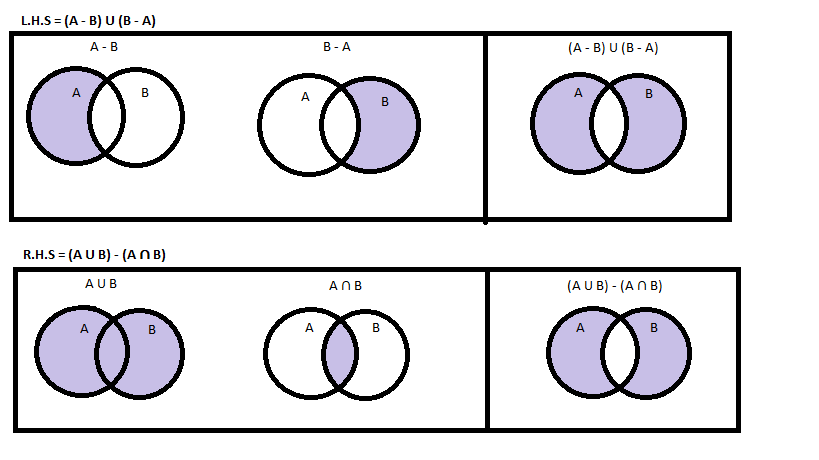
\includegraphics[width=\linewidth]{final12.png}
            \caption{Venn Diagram}
          \label{fig:Venn Diagram}
        \end{figure}
       

    \part[10] For three sets $A, B,$ and $C$ we define the symmetric difference as $A\oplus B\oplus C = (A\oplus B)\oplus C $, meaning using the definition twice. Draw the Venn diagram of this set and express it as in part (a).
    \begin{solution}
         As defined earlier, $A\oplus B = (A \cup B)-(A \cap B)$ \\
         By using the identity proved above, \\
         $A \oplus B \oplus C = (A \cup B)-(A \cap B) \oplus C$ \\
         Again using the same identity: \\
         $A \oplus B \oplus C = [[(A \cup B)-(A \cap B)] \cup C] - [[(A \cup B)-(A \cap B)] \cap C]$
    \end{solution} 
        \begin{figure}[h!]
          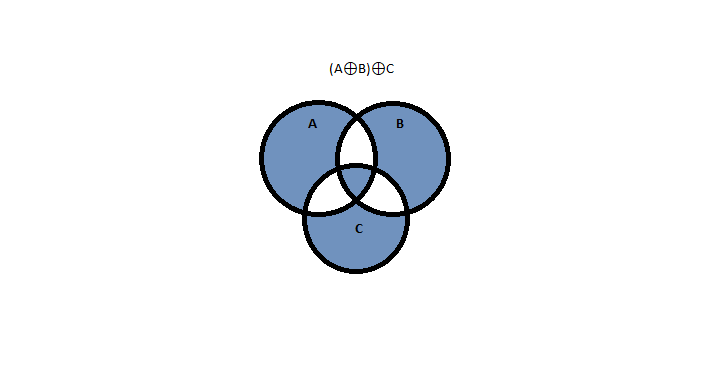
\includegraphics[width=\linewidth]{final22.png}
            \caption{Venn Diagram}
          \label{fig:Venn Diagram}
        \end{figure}
  \end{parts}
   \newpage
  \question
  Let $A$ be the set of all numbers that are divisible by 6 and $B$ the set of all numbers that are divisible by $10$.

  \begin{parts}
    \part[5] Write the sets $A$ and $B$ in proper set notation and describe $A \cap B$ as simply as possible.
    
    \begin{solution}
      $ A = \{\ x \mid x \in x\%6==0 \land x \leq 60 \}$ \\
      $ B = \{\ y \mid y \in y\%10==0 \land y \leq 60 \}$ \\
      $A \cap B$ means all the elements of set A which are also present in set B. \\
      Here, $A \cap B$ is:
      $A \cap B = \{\ 0,30,60 \}$
    \end{solution}
    
    \part[5] What is $A \oplus B$? Describe it using set notation and prove that it is indeed the symmetric difference of $A$ and $B$.
    \begin{solution}
      $A \oplus B=\{\ x \mid x \in A \lor x \in B \land x \notin (A \cap B) \}$ \\
      Where set A is the set of multiples of 6 and set B is the set of multiples of 10.\\
      According to the definition of symmetric difference, it is defined as set of those elements which can be the multiples of 6 or can be the multiples of 10 but cannot be the multiples of both[$ (A \cap B) $] i.e the final set doesn't contain $\{\ 0,30,60... \}$. \\
      Similarly if we find $(A-B) \cup (B-A)$ then according to the given condition set $(A-B)$ would have elements which are multiples of 6 and are not repeated in multiples of 10 i.e $(A-B)= \{\ 6,12,18...\}$. Further we find $(B-A) = \{\ 10,20,..)\}$. Finally the union of both of these will be $(A-B) \cup (B-A) = \{\ 6,12,18,20...\}$ which is equal to the symmetric difference of A and B. \\
      Hence proved,  $A\oplus B = (A-B) \cup (B-A)$
    \end{solution}

    \part[5] List down the elements of $A$, $B$, and $A \oplus B$ if $U = \{x\in \mathcal{N} \mid x \leq 60 \}$.
    \begin{solution}
      $ A = \{\ 0,6,12,18,24,30,36,42,48,54,60\}$ \\
      $ B = \{\ 0,10,20,30,40,50,60 \}$ \\
      $A \oplus B = \{\ 6,10,12,18,20,24,36,40,42,48,50,54 \}$ 
    \end{solution}
  \end{parts}

  \question
  Show that $\overline{ A \cup \overline{B}} = \overline{A} \cap B$.
  \begin{parts}
    
    \part[5] by using set identities.
    \begin{solution}
      Applying De Morgan's Law i.e $\overline{ A \cup B}$= $\overline{A} \cap \overline{B}$ \\ So, $\overline{ A \cup \overline{B}}=\overline{A} \cap \overline{\overline{B}}$ \\ According to the complementation law $ \overline{\overline{B}}$=$B$ \\ Then, $\overline{A} \cap \overline{\overline{B}} =\overline{A} \cap B$ \\
      Hence proved, $\overline{ A \cup \overline{B}} = \overline{A} \cap B$
    \end{solution}
    
    \part[5] by proving that each set is a subset of the other.
    \begin{solution}
      \\ First proving: $\overline{ A \cup \overline{B}}  \subseteq  \overline{A} \cap B$ \\ $x \in \overline{ A \cup \overline{B}}$ \\ $x \notin A \cup \overline{B}$ \\ $x \notin A \lor x \notin \overline{B}$ \\ $x \in \overline{A} \land x \in B$ \\ $x \in \overline{A} \cap B$ 
      \\ Now proving: $ \overline{A} \cap B \subseteq \overline{ A \cup \overline{B}}$ \\ $x \in \overline{A} \cap B$ \\ $ x \in \overline{A} \land x \in B $ \\ $ x \notin A \lor x \notin B $ \\ $ x \notin A \cup \overline{B}$ \\ $ x \in \overline{ A \cup \overline{B}}$
    \end{solution}
  \end{parts}
\end{questions}

\end{document}
